
%%%%%%%%%%%%%%%%%%%%%%%%%%%%%%%%%%%%%%%%%%%%%%%%%%%%%%%%%%%%%%%%%%%%%%%%%%%%%%%%
%%%%%%%%%%%%%%%%%%%%%%%%%%%%%%%%%%%%%%%%%%%%%%%%%%%%%%%%%%%%%%%%%%%%%%%%%%%%%%%%
\section{Procurando um bom ``Timing''}
\label{sec:dancetimming}
\index{Musicalidade!Timing}

\begin{definition}[Timing]
é uma palavra em inglês, que é usada no vocabulario da dança, 
para indicar o grau de exatitude temporal\footnote{%
Sincronização,
sentido de oportunidade \cite{TimingDef}.} 
na execusão de uma sequencia de movimentos.% no momento previsto.
\end{definition}

O Prof. Victor Hugo Suárez dedicado ao ensino de bailes esportivos e danças latinas,
indica que quando falamos que temos um bom timing \cite{TimingDef2} em nossos movimentos de pés, 
nos referimos à capacidade de colocar o peso total do corpo ao principio de cada tempo planejado;
deste jeito estaremos com o peso bem definido e teremos mais tempo 
(o tempo completo entre movimentos  consecutivos), 
para executar corretamente as \hyperref[sec:musicalidade:dinamicas]{\textbf{dinâmicas}} 
planejadas para os movimentos.

Por outro lado os professores Jessie Ma e Clay Boonthanakit
indicam \cite{TimingDef3} que para conseguir uma performance limpa na sua dança,
ter um bom timing, e
um dos fatores\footnote{São indicados 3 fatores para ter uma performance limpa na dança,
estes são: ter um correta posição ou postura em cada movimento, ter um bom timing, e 
acertar o sentimento da música.} importantes a seguir.

\begin{example}
\label{ex:timing1}
Uma pessoa deve executar em bucle, ou reproduzir usando algum software informático,
alguma das sequencias rítmicas descritas na Figura \ref{fig:ex:timing}.
A pessoa que deseja treinar seu timing deve tentar caminhar, ou em geral, 
mexer os pés para acompanhar o ritmo escutado,
ate o ponto de que deve parecer que são os pés da pessoa que executam o ritmo.

Outras indicações para o exercício seriam:
\begin{itemize}
\item Deve-se procurar que o peso do corpo esteja bem definido num pé só 
ao inicio de cada som no ritmo escolhido.
\item Para agregar maior complexidade podem dar palmas em cada tempo forte.
\end{itemize}
\end{example}


\begin{figure}[ht]
\centering
\begin{subfigure}{.475\textwidth}
  \centering
  % include first image
  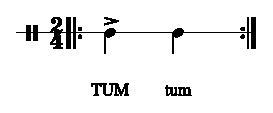
\includegraphics[width=.9\linewidth]{chapters/cap-musicalidade/timing0-1.eps}  
  \caption{Ritmo de treinamento 1.}
  \label{fig:ex:timing:a}
\end{subfigure}
\hfill	
\begin{subfigure}{.475\textwidth}
  \centering
  % include second image
  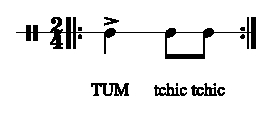
\includegraphics[width=.9\linewidth]{chapters/cap-musicalidade/timing1-1.eps}  
  \caption{Ritmo de treinamento 2.}
  \label{fig:ex:timing:b}
\end{subfigure}

~\\
\vspace{20pt}

\begin{subfigure}{.675\textwidth}
  \centering
  % include second image
  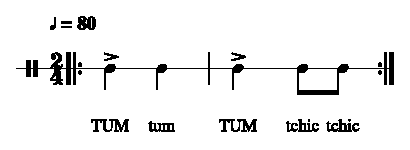
\includegraphics[width=.9\linewidth]{chapters/cap-musicalidade/timing2-1.eps}  
  \caption{Ritmo de treinamento 3.}
  \label{fig:ex:timing:c}
\end{subfigure}
\caption{Possíveis ritmos usados para o treinamento.}
\label{fig:ex:timing}
\end{figure}

O professor de dança Cleidson Diniz propõe \cite{TimingTreino1} 
o exercício descrito no Exemplo \ref{ex:timing:diniz},
\begin{example}
\label{ex:timing:diniz}
Uma pessoa deve jogar ao ar um objeto leve\footnote{A ideia de usar um objeto leve 
é que este não faça barulho ao cair no chão.}, 
e outra pessoa deve bater palmas\footnote{Pode ser trocado por uma pisada forte.}, 
uma vez, no momento exato que este chegue ao chão.
Este exercício pode ser variado tendo em conta o seguinte.
\begin{itemize}
\item A pessoa que vai bater as palmas vê em todo momento a trajetória do objeto.
\item A pessoa que vai bater as palmas só vê o inicio da trajetória. 
Pois o objeto é jogado na sua frente para suas costas.
\item A pessoa que vai bater palmas está com os olhos fechados
e segurando o braço da pessoa que joga o objeto,
de modo que a única informação que tem, 
para predizer o momento do contato do objeto com o chão, 
é o movimento do braço. 
\end{itemize}
\end{example}

%%%%%%%%%%%%%%%%%%%%%%%%%%%%%%%%%%%%%%%%%%%%%%%%%%%%%%%%%%%%%%%%%%%%%%%%%%%%%%%%
%%%%%%%%%%%%%%%%%%%%%%%%%%%%%%%%%%%%%%%%%%%%%%%%%%%%%%%%%%%%%%%%%%%%%%%%%%%%%%%%
% variar el timing implica trabalhar com dinamicas


